\documentclass[a4paper,14pt]{extarticle}

\usepackage[utf8x]{inputenc}
\usepackage[T1,T2A]{fontenc}
\usepackage[russian]{babel}
\usepackage{hyperref}
\usepackage{indentfirst}
\usepackage{here}
\usepackage{array}
\usepackage{graphicx}
\usepackage{caption}
\usepackage{subcaption}
\usepackage{chngcntr}
\usepackage{amsmath}
\usepackage{amssymb}
\usepackage{pgfplots}
\usepackage{pgfplotstable}
\usepackage[left=2cm,right=2cm,top=2cm,bottom=2cm,bindingoffset=0cm]{geometry}
\usepackage{multicol}
\usepackage{askmaps}
\usepackage{titlesec}
\usepackage{listings}
\usepackage{color}
\usepackage{courier}

\definecolor{green}{rgb}{0,0.6,0}
\definecolor{gray}{rgb}{0.5,0.5,0.5}
\definecolor{purple}{rgb}{0.58,0,0.82}

\lstset{
	language=Verilog,
	backgroundcolor=\color{white},   
	basicstyle=\small\ttfamily,
	commentstyle=\color{green},
	keywordstyle=\color{blue},	
	numberstyle=\tiny\color{gray},
	stringstyle=\color{purple},
	breakatwhitespace=false,
	breaklines=true,
	captionpos=b,
	keepspaces=true,
	numbers=left,
	numbersep=5pt,
	showspaces=false,
	showstringspaces=false,
	showtabs=false,
	tabsize=4,
	frame=single,
	inputpath={../quartus/},
	literate={~} {$\sim$}{1}
}

\renewcommand{\le}{\ensuremath{\leqslant}}
\renewcommand{\leq}{\ensuremath{\leqslant}}
\renewcommand{\ge}{\ensuremath{\geqslant}}
\renewcommand{\geq}{\ensuremath{\geqslant}}
\renewcommand{\epsilon}{\ensuremath{\varepsilon}}
\renewcommand{\phi}{\ensuremath{\varphi}}
\renewcommand{\thefigure}{\arabic{figure}} 	
\renewcommand*\not[1]{\overline{#1}}

\titleformat*{\section}{\large\bfseries} 
\titleformat*{\subsection}{\normalsize\bfseries} 
\titleformat*{\subsubsection}{\normalsize\bfseries} 
\titleformat*{\paragraph}{\normalsize\bfseries} 
\titleformat*{\subparagraph}{\normalsize\bfseries} 

\counterwithin{figure}{section}
\counterwithin{equation}{section}
\counterwithin{table}{section}
\newcommand{\sign}[1][5cm]{\makebox[#1]{\hrulefill}}
\graphicspath{{../pics/}}
\captionsetup{justification=centering,margin=1cm}
\def\arraystretch{1.3}
\setlength\parindent{5ex}
\titlelabel{\thetitle.\quad}

\begin{document}

\begin{titlepage}
\begin{center}
	Санкт-Петербургский Политехнический Университет Петра Великого\\[0.3cm]
	Институт компьютерных наук и технологий \\[0.3cm]
	Кафедра компьютерных систем и программных технологий\\[4cm]
	
	\textbf{ОТЧЕТ}\\ 
	\textbf{по лабораторной работе}\\[0.5cm]
	\textbf{SystemVerilog №4}\\[0.1cm]
	Автоматизация проектирования\\ дискретных устройств\\[4.0cm]
\end{center}

\begin{flushright}
	\begin{minipage}{0.45\textwidth}
		\textbf{Работу выполнил студент}\\[3mm]
		группа 33501/4 \hspace*{9mm} Дьячков В.В.\\[5mm]
		\textbf{Преподаватель}\\[5mm]
		\sign[1.5cm] \hspace*{1mm} к.т.н., доц. Филиппов А.С. \\[5mm]
	\end{minipage}
\end{flushright}

\vfill

\begin{center}
	Санкт-Петербург\\
	\the\year
\end{center}
\end{titlepage}

\addtocounter{page}{1}
\counterwithin{lstlisting}{section}

\tableofcontents
\listoffigures
\lstlistoflistings
\newpage

\section{Задачи работы}

\begin{enumerate}
	\setlength\itemsep{0em}
	\item Задание требований к тактовой частоте проекта.
	\item Работа с приложением TimeQuest.
	\item Анализ полученных результатов для максимальной тактовой частоты работы устройства.
\end{enumerate}

\section{Синтез схемы из 2 каскадно-соединенных счетчиков}

\subsection{Результаты синтеза}

На рис. \ref{fig:counter} изображена синтезированная схема, состоящая из 2 каскадно-соединенных счетчиков.

\begin{figure}[H]
\begin{center}
	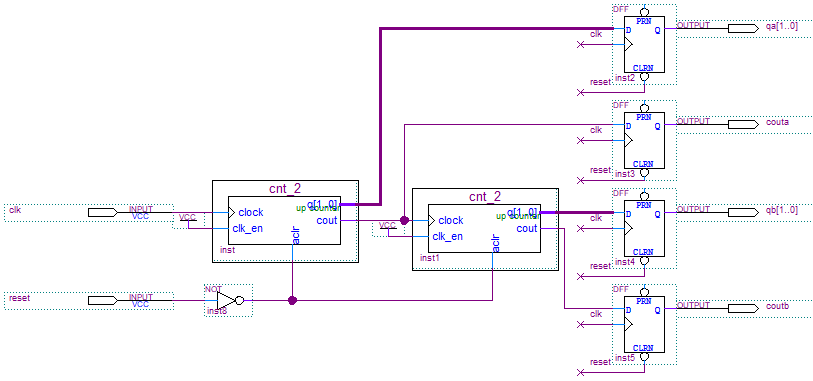
\includegraphics[width=\textwidth]{counter}
	\caption{Синтезированная схема}
	\label{fig:counter}
\end{center}
\end{figure}

\subsection{Результаты компиляции}

В результате компиляции были получены следующие предупреждения от Design Assistant:
\begin{enumerate}
	\setlength\itemsep{0em}
	\item (High) \textbf{Rule C102}: Logic cell should not be used to generate an inverted clock signal.
	\item (High) \textbf{Rule D101}: Data bits are not synchronized when transferred between asynchronous clock domains.
	\item (Medium) \textbf{Rule C103}: Gated clock does not feed at least a pre-defined number of clock ports to effectively save power.
	\item (Medium) \textbf{Rule C104}: Clock signal source should drive only clock input ports.
	\item (Medium) \textbf{Rule R102}: External reset signals should be synchronized using two cascaded registers. 
	\item (Information) \textbf{Rule T102}: Top nodes with the highest number of fan-outs.
\end{enumerate}

\subsection{Результаты синтеза исправленной схемы}

На рис. \ref{fig:counter_right} изображена исправленная схема.

\begin{figure}[H]
\begin{center}
	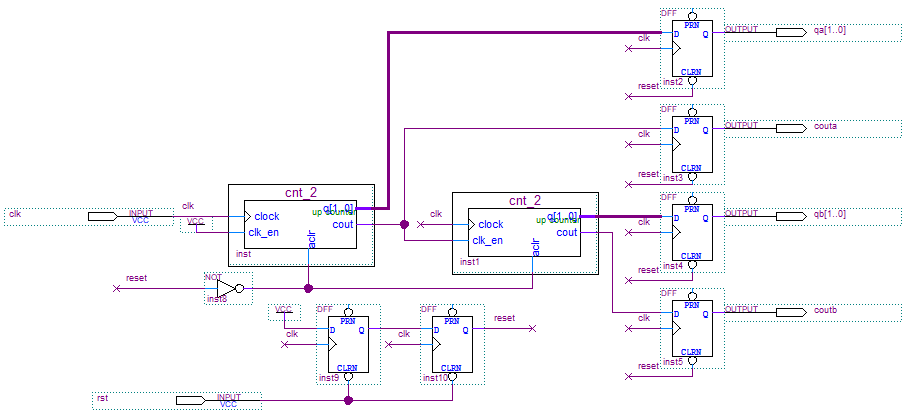
\includegraphics[width=\textwidth]{counter_right}
	\caption{Исправленная схема}
	\label{fig:counter_right}
\end{center}
\end{figure}

\subsection{Результаты компиляции исправленной схемы}

В результате компиляции схемы, изображенной на рис. \ref{fig:counter_right}, было получено только информационное предупреждение \textbf{Rule T102}: Top nodes with the highest number of fan-outs. 

\subsection{Результаты моделирования}

На рис. \ref{fig:modeling} изображен результат функционального моделирования. Из временной диаграммы видно, что схема из 2 каскадно-соединенных счетчиков синтезирована верно.

\begin{figure}[H]
\begin{center}
	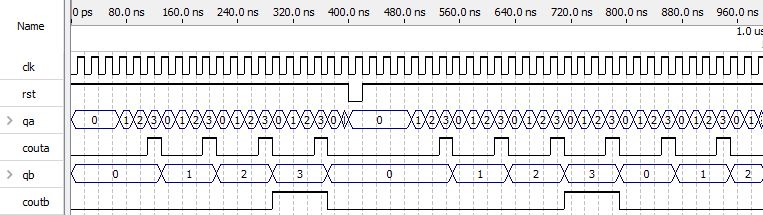
\includegraphics[width=\textwidth]{modeling}
	\caption{Результаты моделирования}
	\label{fig:modeling}
\end{center}
\end{figure}

%TODO На выходе qa новое значение счетчика (1) появляется только на 4 такте после того, как сигнал асинхронного сброса был снят?
%TODO В самом начале моделирования значение 0 присутствует на выходе 4 такта?

\subsection{Создание SDC файла}

В листинге \ref{code:sdc} приведена сформированная SDC команда, создающая ограничения для тактового сигнала.

\begin{lstlisting}[caption=Synopsys Design Constraints (SDC) файл, label=code:sdc]
create_clock -name input_clk -period 20.000 [get_ports {clk}]
derive_clock_uncertainty
\end{lstlisting}

\subsection{Результаты временного анализа}

В отчете компиляции в разделе \textbf{TimeQuest Timing Analyzer} указана максимальная тактовая частота работы проекта: Fmax = $335.68$ MHz, Restricted Fmax = $250.0$ MHz. Следовательно требование к максимальной тактовой частоте выполнено. При этом максимальная частота работы проекта равна $335.68$ MHz.

\newpage

\section{Синтез схемы из 3 каскадно-соединенных счетчиков}

\subsection{Результаты синтеза}

На рис. \ref{fig:counter_three} изображена синтезированная схема, состоящая из 3 каскадно-соединенных счетчиков.

\begin{figure}[H]
\begin{center}
	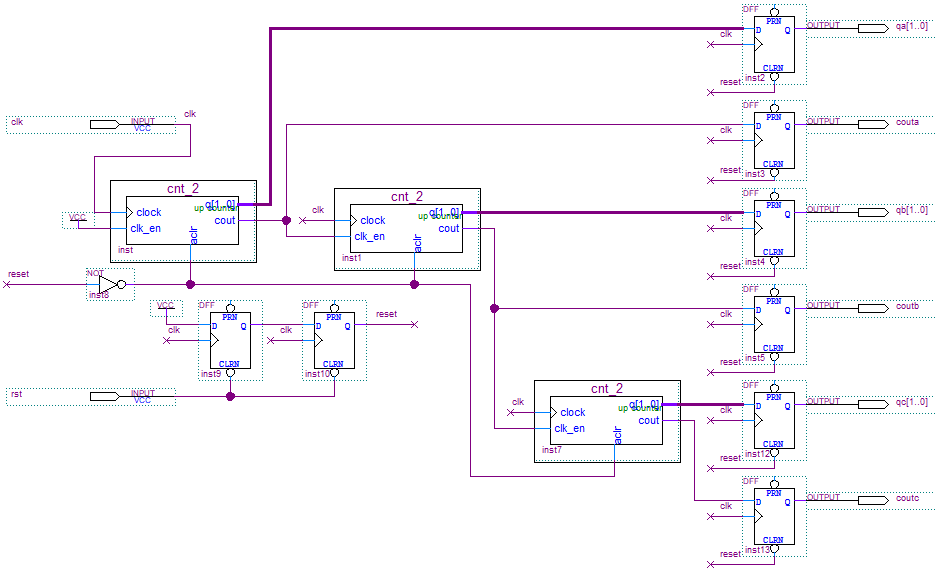
\includegraphics[width=\textwidth]{counter_three}
	\caption{Синтезированная схема}
	\label{fig:counter_three}
\end{center}
\end{figure}

\subsection{Результаты компиляции}

В результате компиляции данной схемы было получено только информационное предупреждение \textbf{Rule T102}: Top nodes with the highest number of fan-outs.

\subsection{Результаты моделирования}

На рис. \ref{fig:counter_three_modeling} изображен результат функционального моделирования. Из временной диаграммы видно, что схема из 3 каскадно-соединенных счетчиков синтезирована верно.

\begin{figure}[H]
\begin{center}
	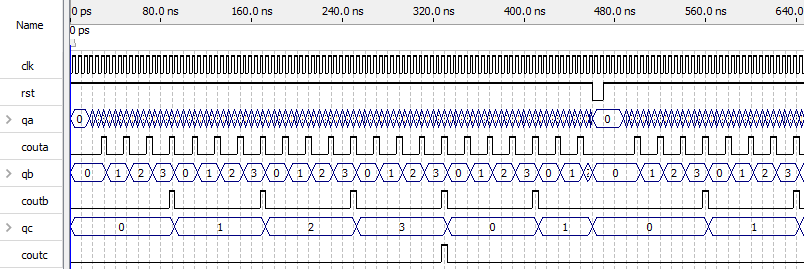
\includegraphics[width=\textwidth]{counter_three_modeling}
	\caption{Результаты моделирования}
	\label{fig:counter_three_modeling}
\end{center}
\end{figure}

\subsection{Результаты временного анализа}

В отчете компиляции в разделе \textbf{TimeQuest Timing Analyzer} указана максимальная тактовая частота работы проекта: Fmax = $200.48$ MHz, Restricted Fmax = $200.48$ MHz. Следовательно требование к максимальной тактовой частоте выполнено. При этом максимальная частота работы проекта равна $200.48$ MHz.

\section{Выводы}

%TODO вывод

\end{document}